%Photoshop techniques for changing skintone from select online video tutorials
\subsection{Changing skin colour from dark to light \cite{photoshop:obama}}\label{app:photoshop_obama}
\begin{longtable}{|c|c|}
    \caption{Screen captures from Photoshop tutorial for changing skin colour from dark to light.}\\
    \hline
    Original & Result \\
    \hline
  \begin{minipage}{.29\textwidth}
    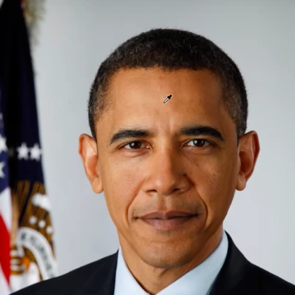
\includegraphics[width=\textwidth,height=\textheight,keepaspectratio]{images/obama_orig}
  \end{minipage} & 
  \begin{minipage}{.29\textwidth}
    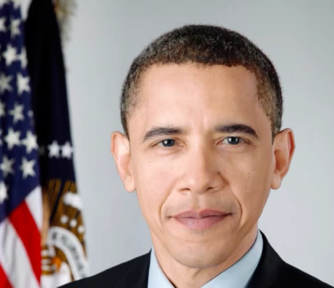
\includegraphics[width=\textwidth,height=\textheight,keepaspectratio]{images/obama_res}
  \end{minipage} \\
    \hline
\end{longtable}
\pagebreak

\subsection{Matching the skintones of face and body \cite{photoshop:match_body}}\label{app:photoshop_match_body}
\begin{longtable}{|c|c|c|}
    \caption{Screen captures from Photoshop tutorial for matching the skintones of face and body.}\\
    \hline
    Original & Target & Result \\
    \hline
  \begin{minipage}{.29\textwidth}
    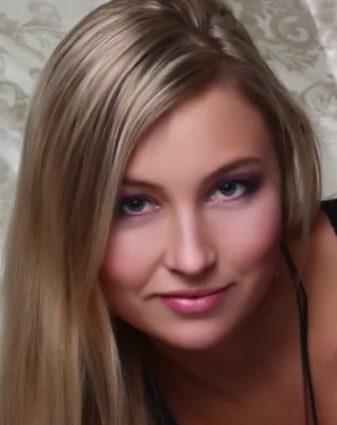
\includegraphics[width=\textwidth,height=\textheight,keepaspectratio]{images/match_body_orig}
  \end{minipage} & 
  \begin{minipage}{.29\textwidth}
    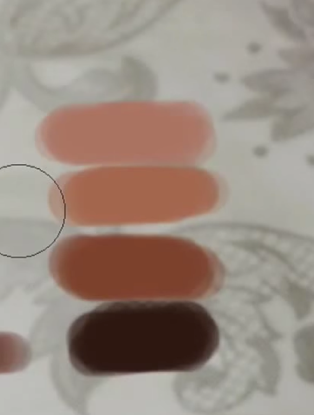
\includegraphics[width=\textwidth,height=\textheight,keepaspectratio]{images/match_body_targ}
  \end{minipage} & 
  \begin{minipage}{.29\textwidth}
    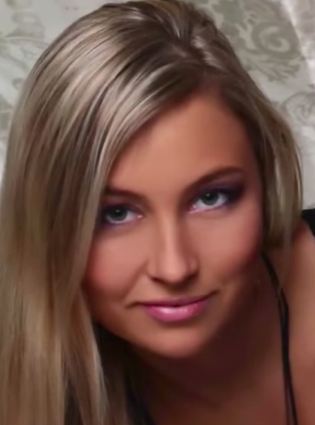
\includegraphics[width=\textwidth,height=\textheight,keepaspectratio]{images/match_body_res}
  \end{minipage} \\
    \hline
\end{longtable}
\pagebreak

\subsection{Matching the skintones of portraits of different people \cite{photoshop:match_other} }\label{app:photoshop_match_other}
\begin{longtable}{|N||c|c|c|}
    \caption{Screen captures from Photoshop tutorial for matching the skintones of portraits of different people.}\\
    \hline
    \multicolumn{1}{|c||}{No.} & Original & Target & Result \\
    \hline  \label{row:photoshop_match_other_1} &
  \begin{minipage}{.29\textwidth}
    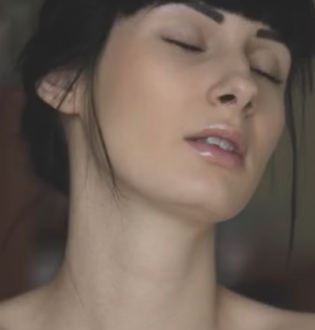
\includegraphics[width=\textwidth,height=\textheight,keepaspectratio]{images/match_other_1_orig}
  \end{minipage} & 
  \begin{minipage}{.29\textwidth}
    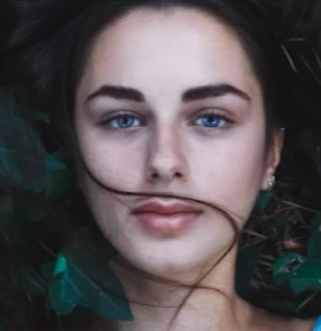
\includegraphics[width=\textwidth,height=\textheight,keepaspectratio]{images/match_other_1_targ}
  \end{minipage} & 
  \begin{minipage}{.29\textwidth}
    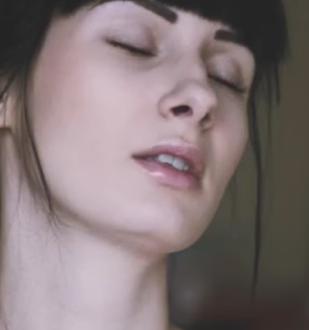
\includegraphics[width=\textwidth,height=\textheight,keepaspectratio]{images/match_other_1_res}
  \end{minipage} \\
    \hline  \label{row:photoshop_match_other_2} &
  \begin{minipage}{.29\textwidth}
    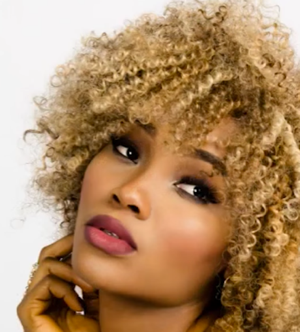
\includegraphics[width=\textwidth,height=\textheight,keepaspectratio]{images/match_other_2_orig}
  \end{minipage} & 
  \begin{minipage}{.29\textwidth}
    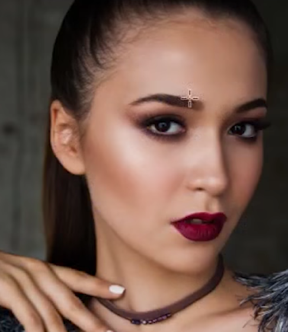
\includegraphics[width=\textwidth,height=\textheight,keepaspectratio]{images/match_other_2_targ}
  \end{minipage} & 
  \begin{minipage}{.29\textwidth}
    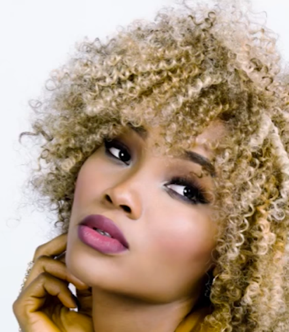
\includegraphics[width=\textwidth,height=\textheight,keepaspectratio]{images/match_other_2_res}
  \end{minipage} \\
    \hline
\end{longtable}